\documentclass[8pt]{beamer}
\usepackage[utf8]{inputenc}

\usetheme{Madrid}

%% ADDITIONAL NICOLÁS
\usepackage{ragged2e}
\usepackage{amssymb}
\usepackage{subcaption}

\usefonttheme{serif}
\definecolor{UBCblue}{rgb}{0.01569, 0.11765, 0.25882} % PSU Blue
\usecolortheme[named=UBCblue]{structure}

%% ADDITIONAL NICOLÁS




%------------------------------------------------------------
%This block of code defines the information to appear in the
%Title page
\title[Lattice Boltzmann Method] %optional
{Lattice Boltzmann Method in Multiphase Transport Phenomena}

\subtitle{Research Overview}

\author[Nicolás Bueno] % (optional)
{Nicolás Bueno\inst{1} \and Advisor: Dr. Ayala\inst{1} \and Co-advisor: Dr. Mehmani\inst{1}}

\institute[EME] % (optional)
{
	\inst{1}%
	Department of Energy and Mineral Engineering\\
	Penn State University\\
	
\includegraphics[height=1cm]{pics/PSU_EMS.png}
}

\date[Spring 2022] % (optional)
{}

%\logo{
\includegraphics[height=1cm]{pics/PSU_EMS.png}}

%End of title page configuration block
%------------------------------------------------------------



%------------------------------------------------------------
%The next block of commands puts the table of contents at the 
%beginning of each section and highlights the current section:

\AtBeginSection[]
{
	\begin{frame}
		\frametitle{Table of Contents}
		\tableofcontents[currentsection]
	\end{frame}
}
%------------------------------------------------------------


\begin{document}
	
	%The next statement creates the title page.
	\frame{\titlepage}
	
	%---------------------------------------------------------
	%This block of code is for the table of contents after
	%the title page
	\begin{frame}
		\frametitle{Table of Contents}
		\tableofcontents
	\end{frame}
	%---------------------------------------------------------
	
	\justifying
	
	\section{Motivation}	
	\begin{frame}{Motivation}
		
		Applications: 
		\begin{itemize}
			\item CO$_2$ mineralization, gas densification, and gas diffusion 
			\item Solute transport and phase distribution
			\item Relative permeabilities - wettability
		\end{itemize}
		
		~\\\textbf{Why a new code?}: 
		\begin{itemize}
			\item 3D version for arbitrary domains, forces, and boundary conditions
			\item Future parallelization
			\item Coupling with other transport equations
		\end{itemize}
		
		~\\~\\Fortran 90, Object Oriented, LBM code for multi-component ($N_c$) mixtures. Output in VTK format.
	\end{frame}

	\section{The Lattice Boltzmann Method - Formulation}
	\begin{frame}[t]
		\frametitle{The Lattice Boltzmann Method - Formulation}
		
		The Lattice Boltzmann Method is based on kinetic theory, that states:
		
		\begin{equation}\label{eq:LBPDE}
			\underbrace{\frac{\partial f_i(x,t)}{\partial t} + \mathbf{c}_i \frac{\partial f_i(x,t)}{\partial x}}_{\text{Streaming - DF Advection}} = \underbrace{\mathbf{\Omega}}_{\text{Collision}} 
		\end{equation}
		
		What in its discretized form\footnote{Going from \ref{eq:LBPDE} to \ref{eq:LBE}, what about spatial derivative?} becomes:
		\begin{equation}\label{eq:LBE}
			f_i(x+ \mathbf{c}_i \Delta t, t+\Delta t) - f_i(x, t) = - \mathbf{M}^{-1} \mathbf{S} [\mathbf{m}(x,t) - \mathbf{m}^{\text{eq}}]  + \hat{F}_i
		\end{equation}
		where $\mathbf{m}$ are vectors of moments, $\mathbf{S}$ is a relaxation diagonal matrix, and $\mathbf{M}$ is a fixed matrix depending on DnQm. $ \mathbf{m}^{\text{eq}} = f(f_i^{\text{eq}}, \mathbf{F})$.
	\end{frame}
	
	
	\begin{frame}
		\frametitle{Macroscopic variables}
		Density and velocity are computed as follows:
		\begin{equation}
			\rho = \sum_i f_i \, \, \, \, \, \, \, \,  \mathbf{u} = \sum_i \mathbf{c}_i f_i
		\end{equation}
		Two important constitutive equations:
		\begin{equation*}
			f_i^{\text{eq}} = \rho \omega_i \left[ 1 + \frac{\vec{u}\cdot \vec{\mathbf{c}_i}}{c^2_s} + \frac{(\vec{u}\cdot \vec{\mathbf{c}_i})^2}{2c^4_s}-  \frac{\vec{u}\cdot \vec{u}}{2c^2_s} \right]
		\end{equation*}
		
		\begin{equation*}
			\hat{F}_i = \frac{\mathbf{F}}{\rho} \frac{\vec{u} - \vec{\mathbf{c}_i}}{c^2_s} f_i^{\text{eq}}  
		\end{equation*}
		
		where $\mathbf{F}$ is defined in the multiphase problem, as the Shan Cheng force:
		\begin{equation}
			\mathbf{F} = -G \psi(x) \sum_i \omega_i \psi(x+\mathbf{c}_i \delta t) \mathbf{c}_i \, \, \, \, \, \psi := \sqrt{\frac{2(P^{\text{\tiny EoS}}-c_s^2\rho)}{G \delta t c_s^2}}
		\end{equation}
	\end{frame}
	
	
	\section{Dynamic Validations}
	\begin{frame}{Dynamic Validations}
		
		The main validation sources are: analytical solutions, Cheng's codes, qualitative physics understanding.\\~\\
		
		
		\begin{columns}[T]
			
			\column{0.5\textwidth}
			Single phase:
			\begin{itemize}
				\item Channel flow ($\mathbf{F}$ \& $\nabla p$-driven)
				\item Couette flow (plates)
				\item Cylinder (turbulent)
				\item Cavity flow
				\item Porous medium
			\end{itemize}
			
			\column{0.5\textwidth}
			Multiphase:
			\begin{itemize}
				\item Static droplet
				\item Oscillation droplet
				\item Falling droplet
			\end{itemize}
		\end{columns}
	\end{frame}
	
	\begin{frame}{Single phase validations (quantitative)}
		\begin{figure}[h]
			\centering
			\begin{subfigure}{.5\textwidth}
				\centering
				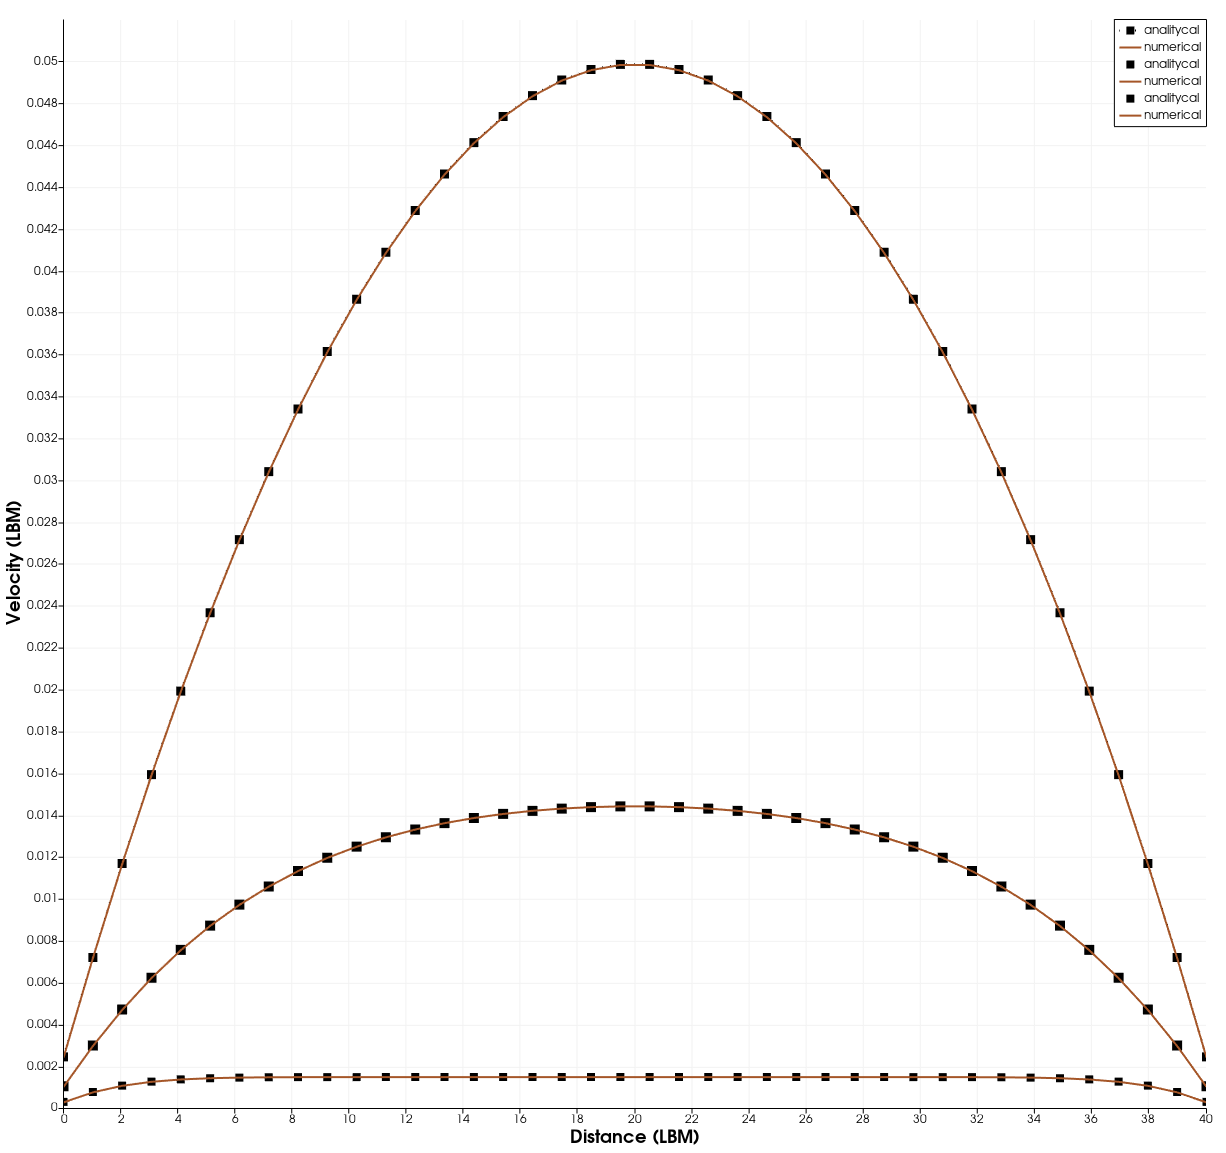
\includegraphics[width=.9\linewidth]{pics/channelForceDrivenValidation.png}
				\caption{$\mathbf{F}$-driven channel flow}
				\label{fig:sub1}
			\end{subfigure}%
			\begin{subfigure}{.5\textwidth}
				\centering
				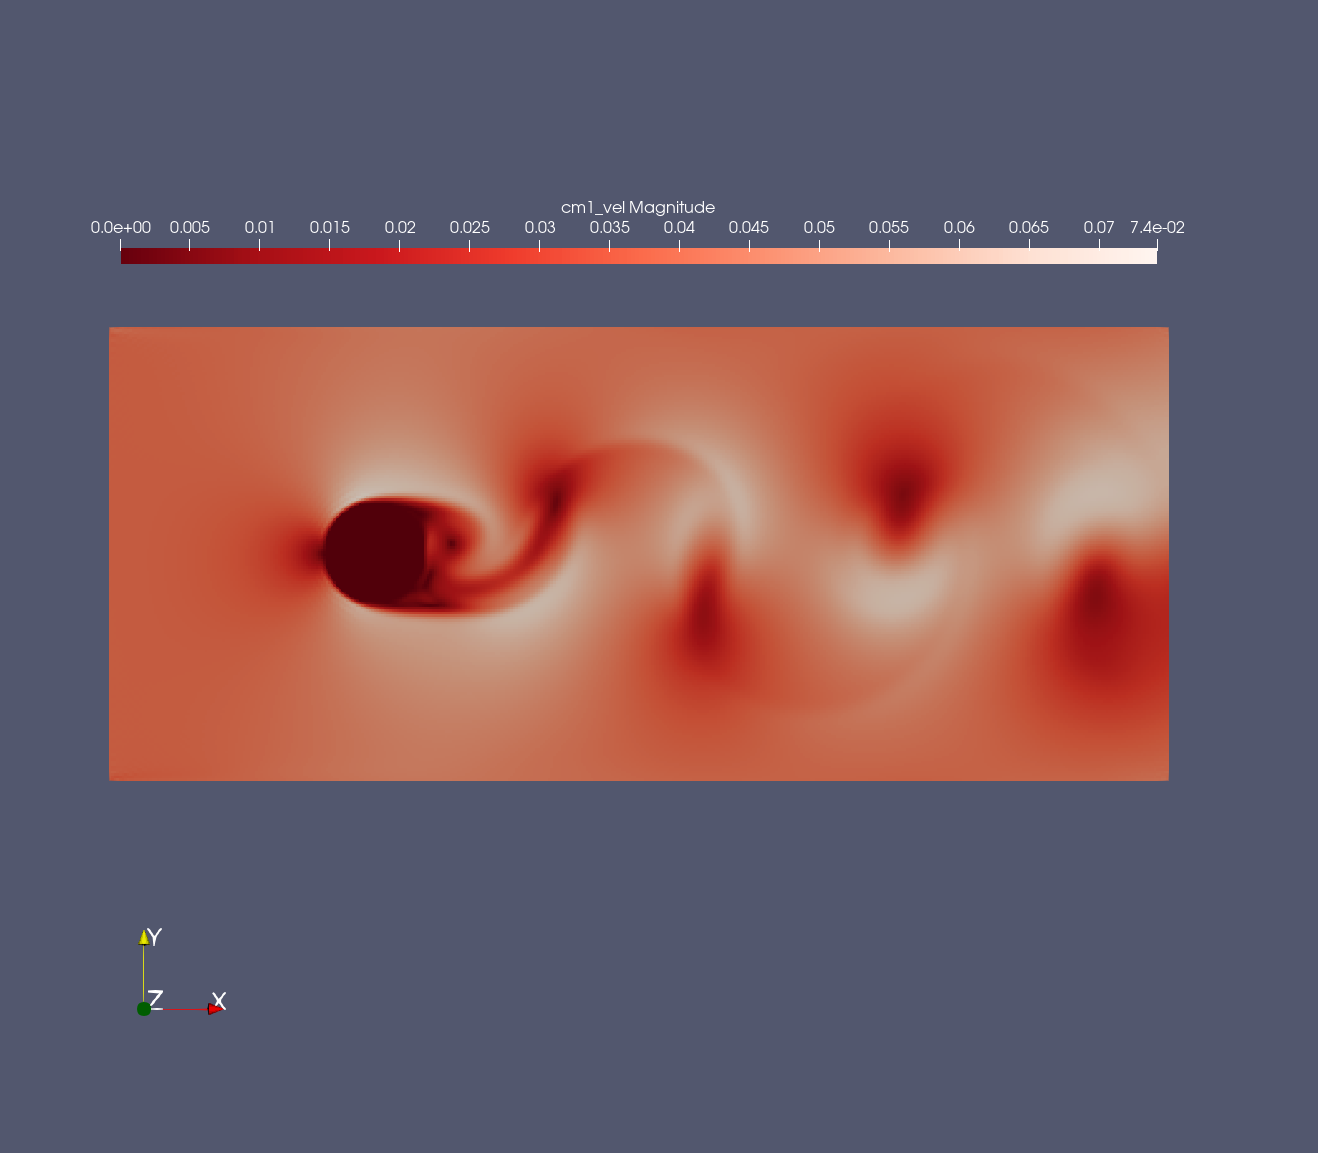
\includegraphics[width=.9\linewidth]{pics/cylinderTurbulent.png}
				\caption{Turbulent flow around cylinder}
				\label{fig:sub2}
			\end{subfigure}
			\caption{Results with direct source for quantitative comparisons.}
			\label{fig:osci}
		\end{figure}
	\end{frame}
	
	\begin{frame}{Single phase validations (qualitative)}
		\begin{figure}[h]
			\centering
			\begin{subfigure}{.5\textwidth}
				\centering
				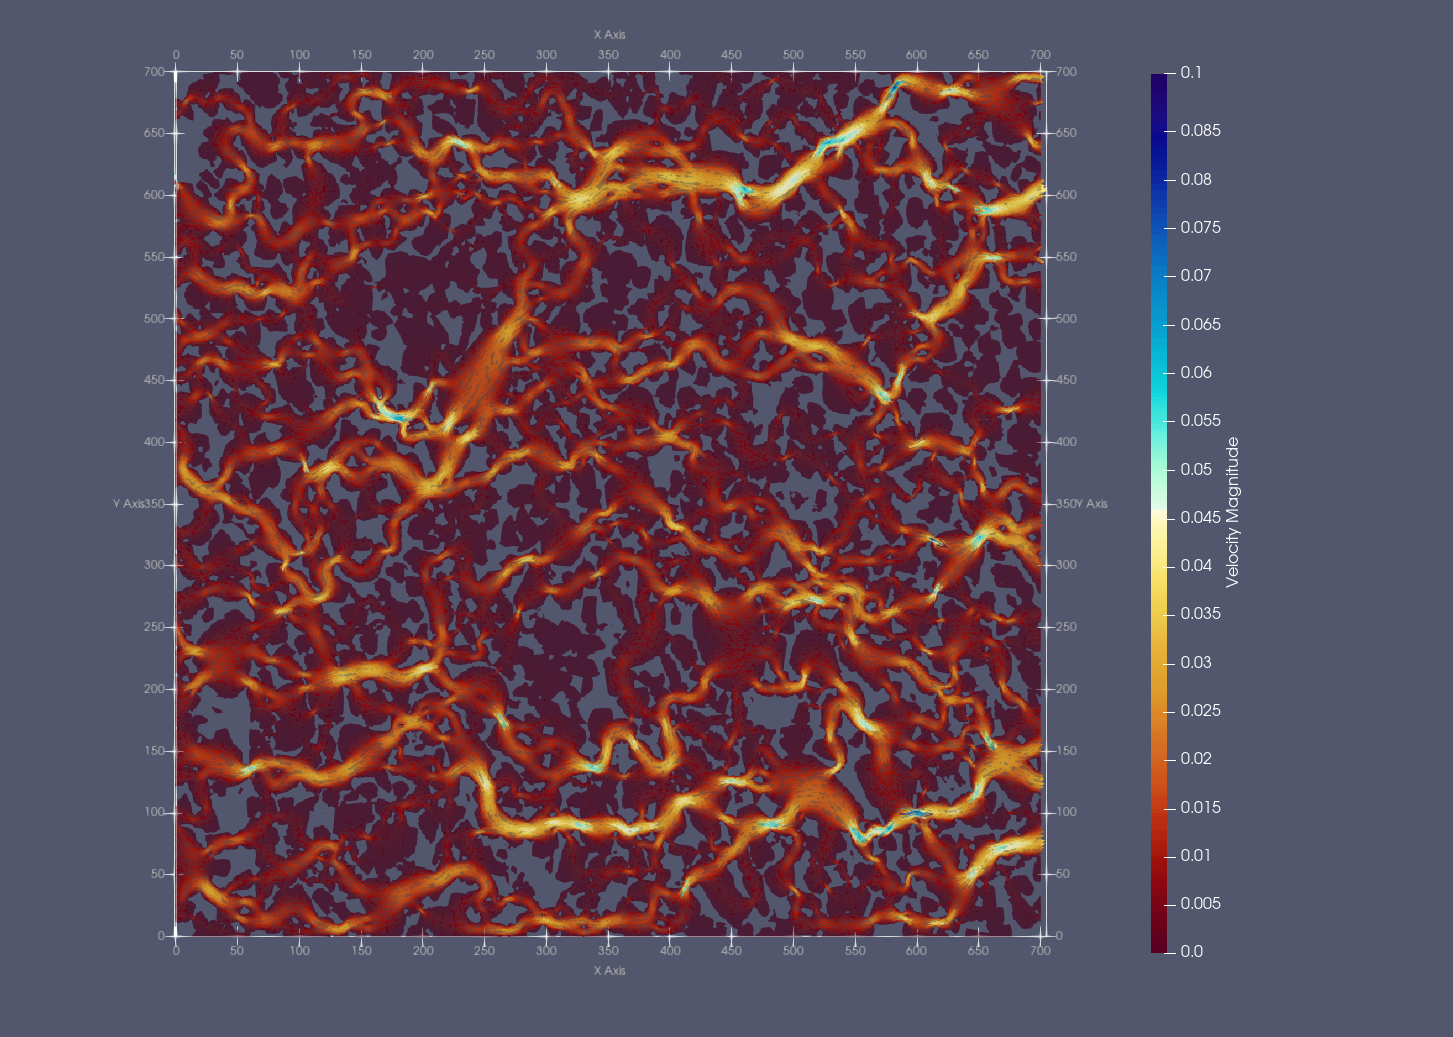
\includegraphics[width=.9\linewidth]{pics/pmVelLowV.png}
				\caption{Arbitrary porous medium (real image).}
		
			\end{subfigure}%
			\begin{subfigure}{.5\textwidth}
				\centering
				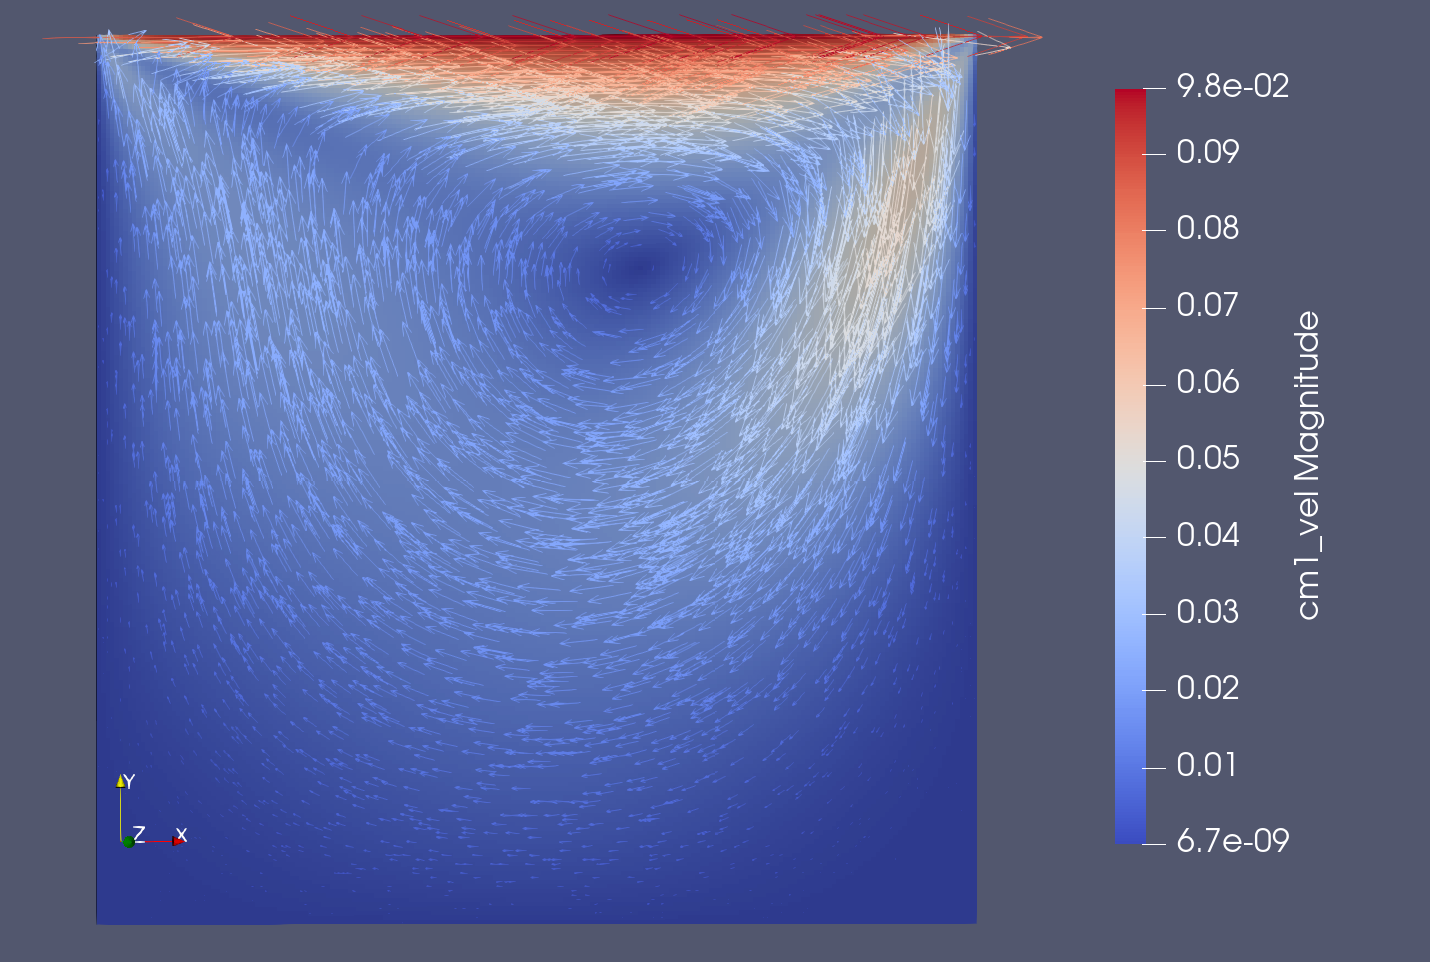
\includegraphics[width=.9\linewidth]{pics/cavity.png}
				\caption{Cavity flow, imposing a velocity on the upper wall.}
		
			\end{subfigure}
			\caption{Single phase cases qualitatively demonstrating the ability of modeling arbitrary porous media and arbitrary boundary conditions.}
	
		\end{figure}
	\end{frame}
	
	\begin{frame}{Multiphase single component - Oscillating droplet}
		\begin{figure}[h]
			\centering
			\begin{subfigure}{.5\textwidth}
				\centering
				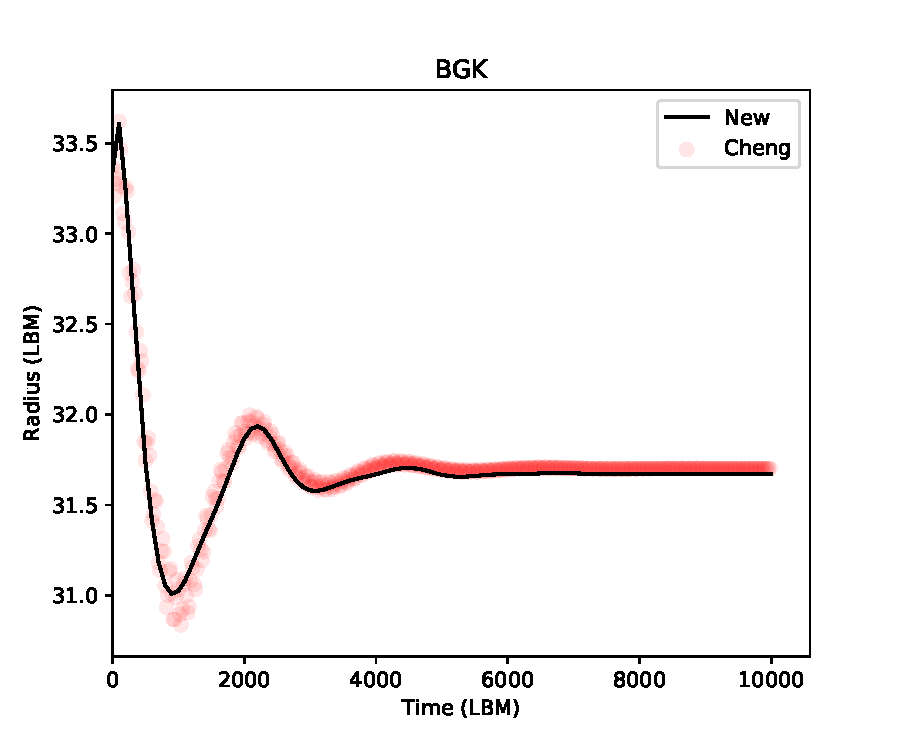
\includegraphics[width=.9\linewidth]{pics/BGKOsc.pdf}
				\caption{BGK}
	
			\end{subfigure}%
			\begin{subfigure}{.5\textwidth}
				\centering
				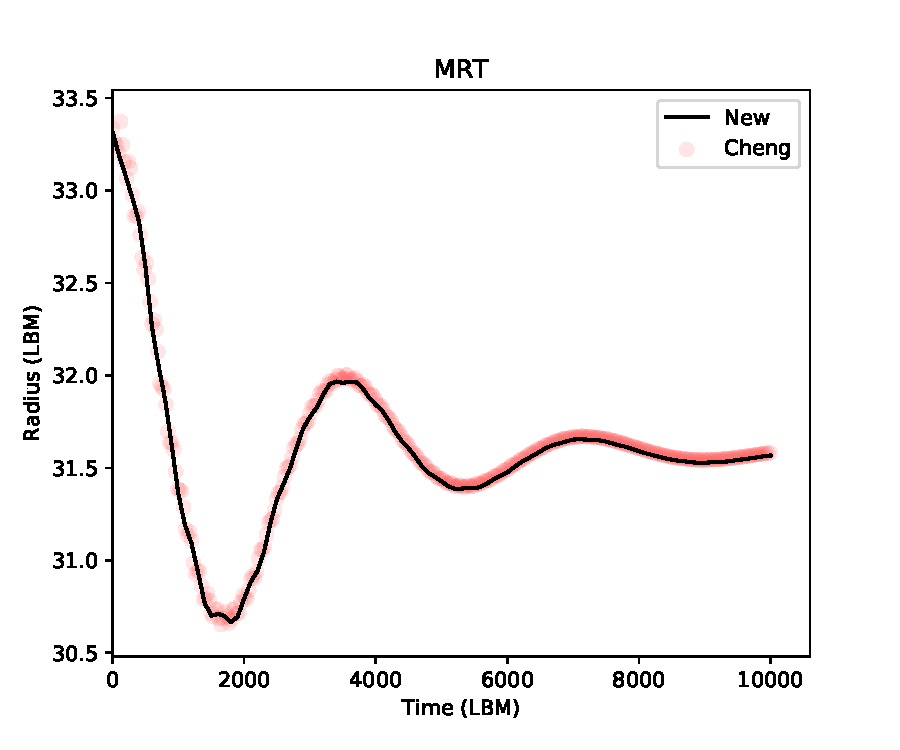
\includegraphics[width=.9\linewidth]{pics/MRTOsc.pdf}
				\caption{MRT}

			\end{subfigure}
			\caption{Oscillation droplet case. Viscosities are different in each case.}
		\end{figure}
	\end{frame}
	
	
		\begin{frame}{Static results - Young Laplace}
		$P_c = \frac{\sigma}{r}$, for a 2D geometry.
		$\sigma = $ 0.12141. Here, $r = R_e$, the equilibrium radius.
		
		\begin{figure}[h]
			\centering
			\begin{subfigure}{.5\textwidth}
				\centering
				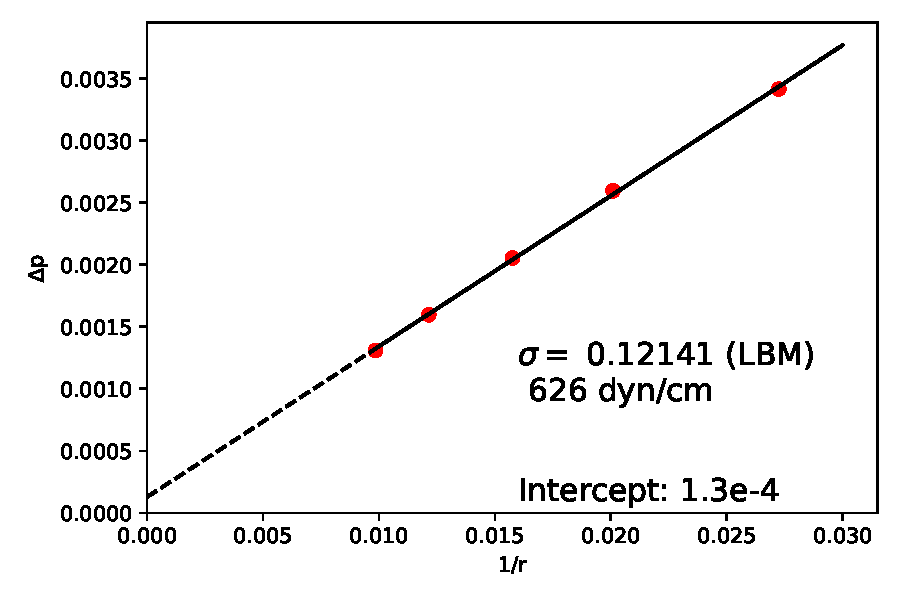
\includegraphics[width=1\linewidth]{pics/IFT.pdf}
				\caption{Young-Laplace validation}
			\end{subfigure}%
			\begin{subfigure}{.5\textwidth}
				\centering
				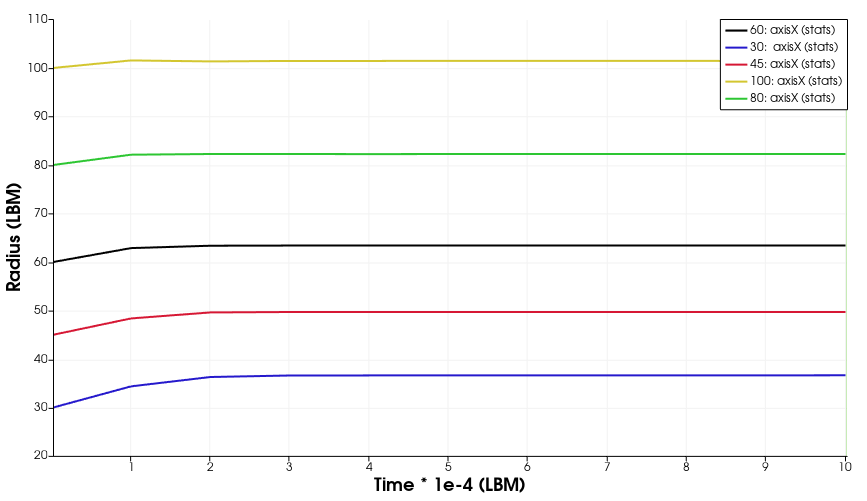
\includegraphics[width=1\linewidth]{pics/2c_staticRChange.png}
				\caption{Evolution of $R_e$ for the static cases.}
			\end{subfigure}
			\caption{Young Laplace and $R_e$ change due to thermodynamic inconsistency.}
			\label{fig:laplace}
		\end{figure}
		
	\end{frame}
	
	\begin{frame}{Oscillating droplet}
		$R_{x,0} = 60, R_{y,0} = 0.9 R_{x,0}$, in a grid of 400x400. $\tau_l = \tau_v = 0.56$, to reduce the viscous dissipation.
		\begin{figure}[h]
			\centering
			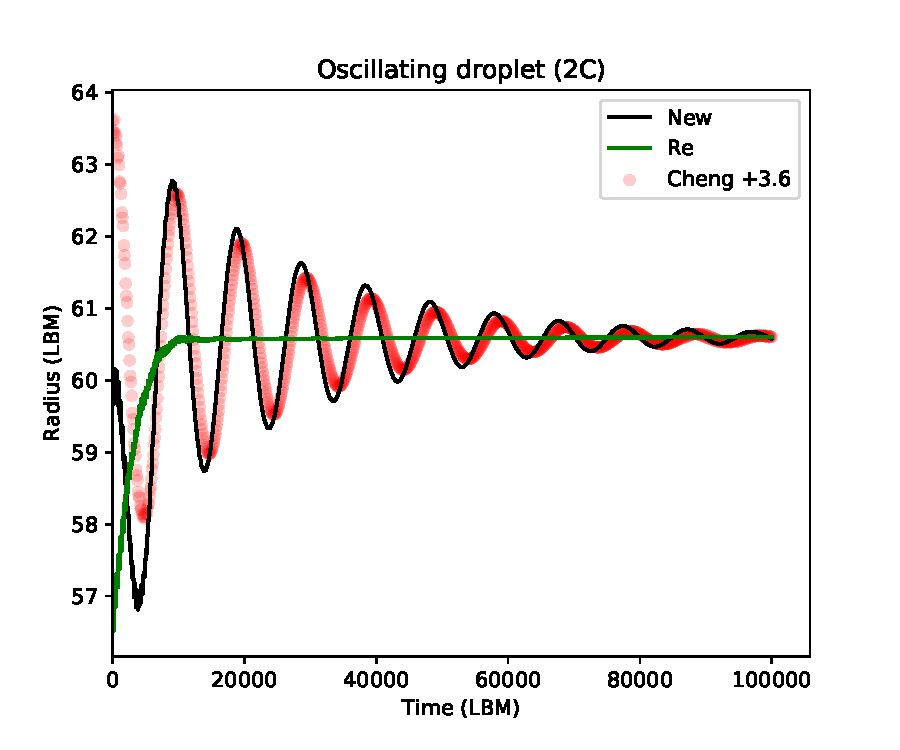
\includegraphics[scale=0.4]{pics/2cOsc.pdf}
			\caption{Oscillation of the X axis compared with Cheng's solution.}
			\label{fig:2cOsc}
		\end{figure}
	\end{frame}
	
	\begin{frame}{Fourier transform}
		
		\begin{columns}
			
			\column{0.5\textwidth}
			\begin{figure}[h]
				\centering
				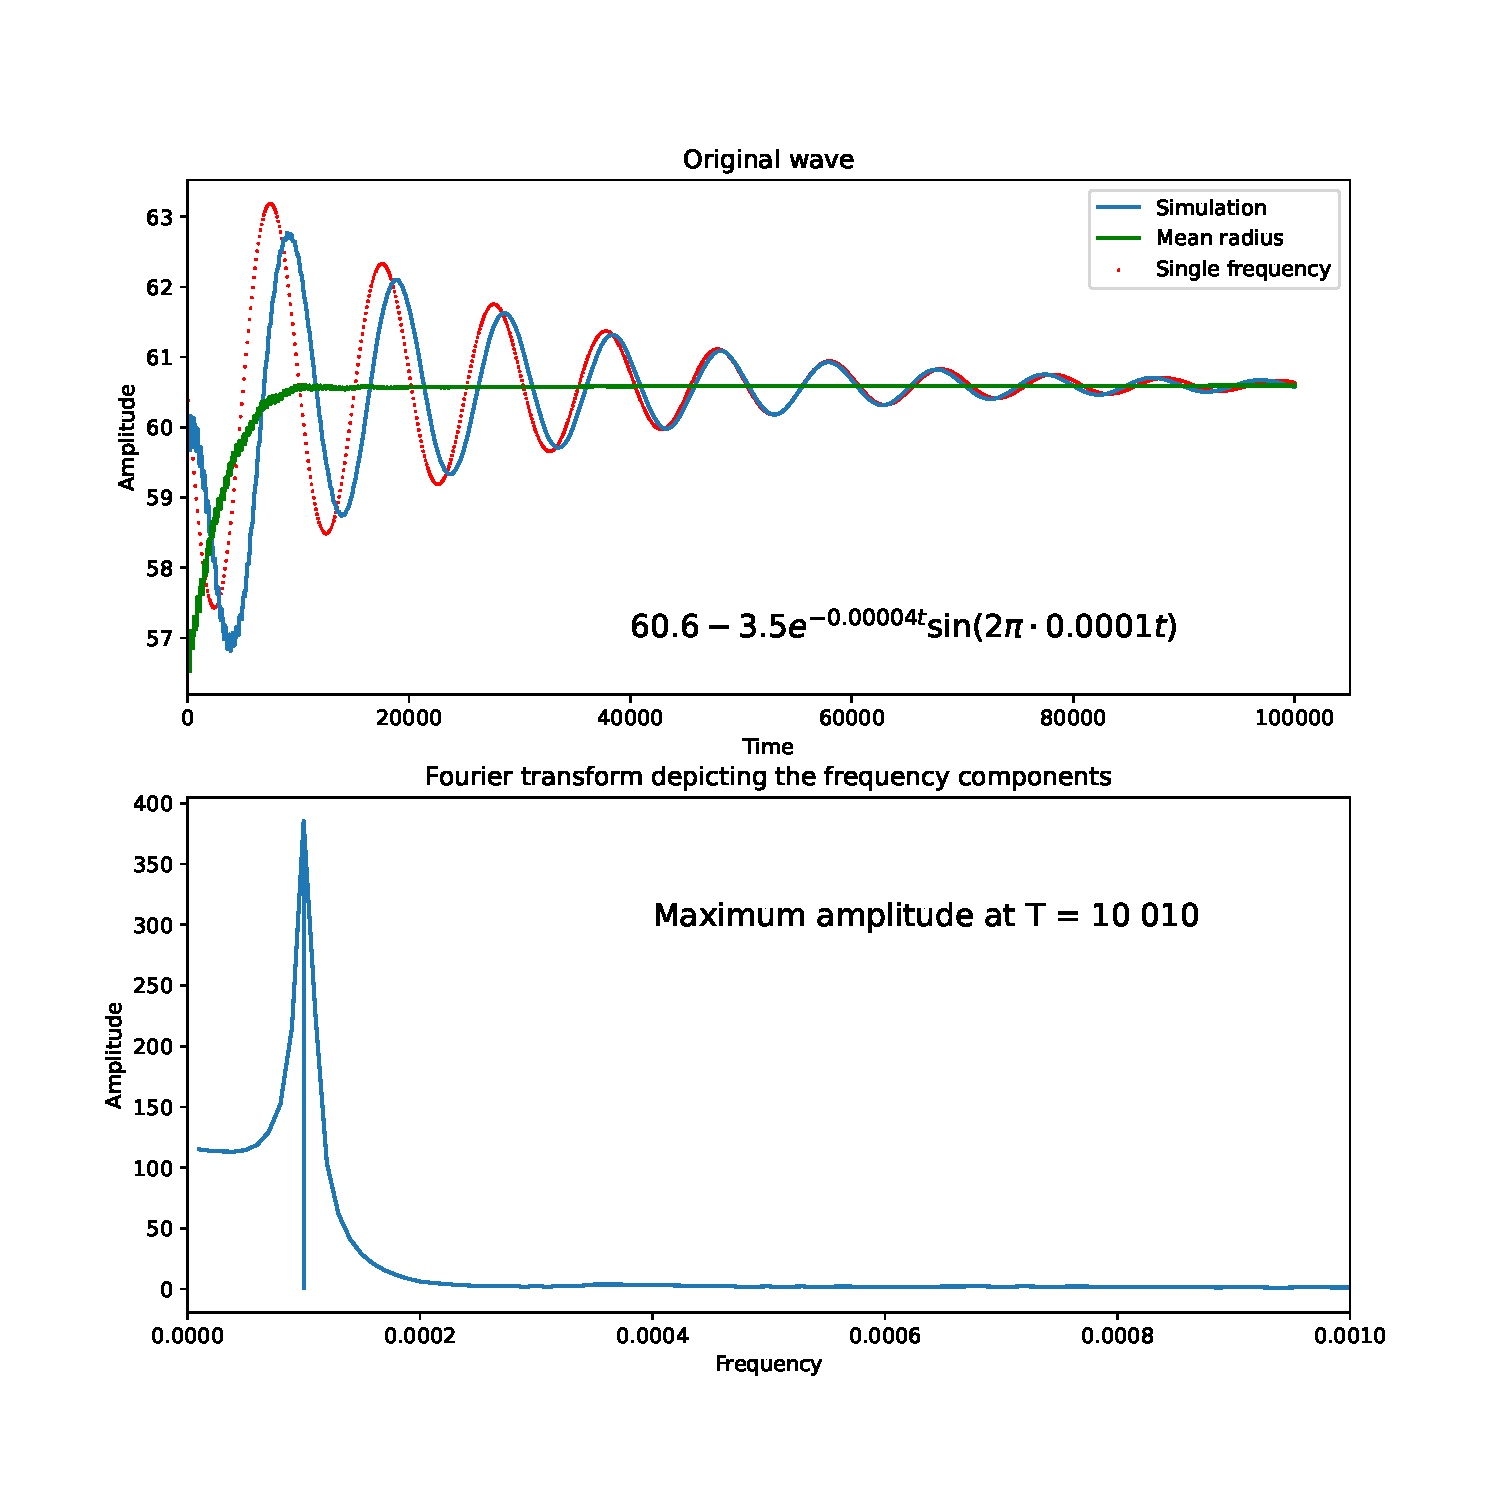
\includegraphics[width=1\linewidth]{pics/fourier.pdf}
				\caption{Maximum amplitude at $T_n = 10010$.}
				\label{fig:2cOsc}
			\end{figure}
			
			\column{0.5\textwidth}
			Analytical solution:
			\begin{equation}
				T_a = 2 \pi \left[ \frac{n (n^2-1) \sigma}{\rho_l R_e^3} \right]^{-0.5}
			\end{equation}
			Giving a period $T_a = $ 9989. This gives a relative error of 2\%. 
		\end{columns}	
	\end{frame}
	
	\section{Ongoing work}
	\begin{frame}{Ongoing work - Raising bubble physics}
		    
		\begin{columns}[T]
			
			\column{0.5\textwidth}
			
			\begin{itemize}
				\item Main properties
				\begin{itemize}
					\item Surface tension
					\item Body forces
					\item Viscosity and density ratio
					\item Boundary conditions
				\end{itemize}
				
				\item Bond and Morton numbers fix $R_e = \frac{u_t d_b}{\nu_l}$
				\begin{equation*}
					\begin{split}
						B_o = \frac{g \Delta \rho d_b^2}{\sigma}\\
						M_o = \frac{g \Delta \rho \mu_l^4}{\sigma^3 
							\rho_l^2}
					\end{split}
				\end{equation*}
				
				\item The drag coefficient, $C_D$, function of $R_e$, and defined as: 
				\begin{equation*}
					\begin{split}
						C_D = \frac{4 \Delta \rho g d_b}{3 u_t^2 \rho_l}
					\end{split}
				\end{equation*}
				resulting from a drag and gravity force balance. 
			\end{itemize}
			
			\column{0.5\textwidth}
			\begin{figure}
				\centering
				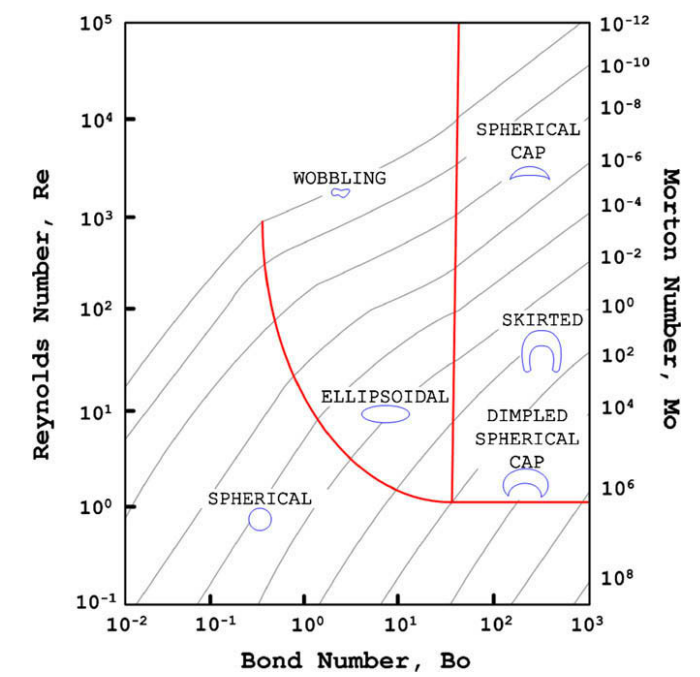
\includegraphics[scale=0.2]{pics/shapeRegimes.png}
				\\{\tiny \justifying Taken from Amaya-Bower L., Lee T. Single bubble rising dynamics for moderate Reynolds number using Lattice Boltzmann Method. Computer and Fluids. 2010.}
			\end{figure}
			
		\end{columns}
		
	\end{frame}
	
	\begin{frame}{Experimental relationship of $C_D$ with $R_e$}
		
		The constants may change due to the 2D approximation. 
		\begin{figure}
			\centering
			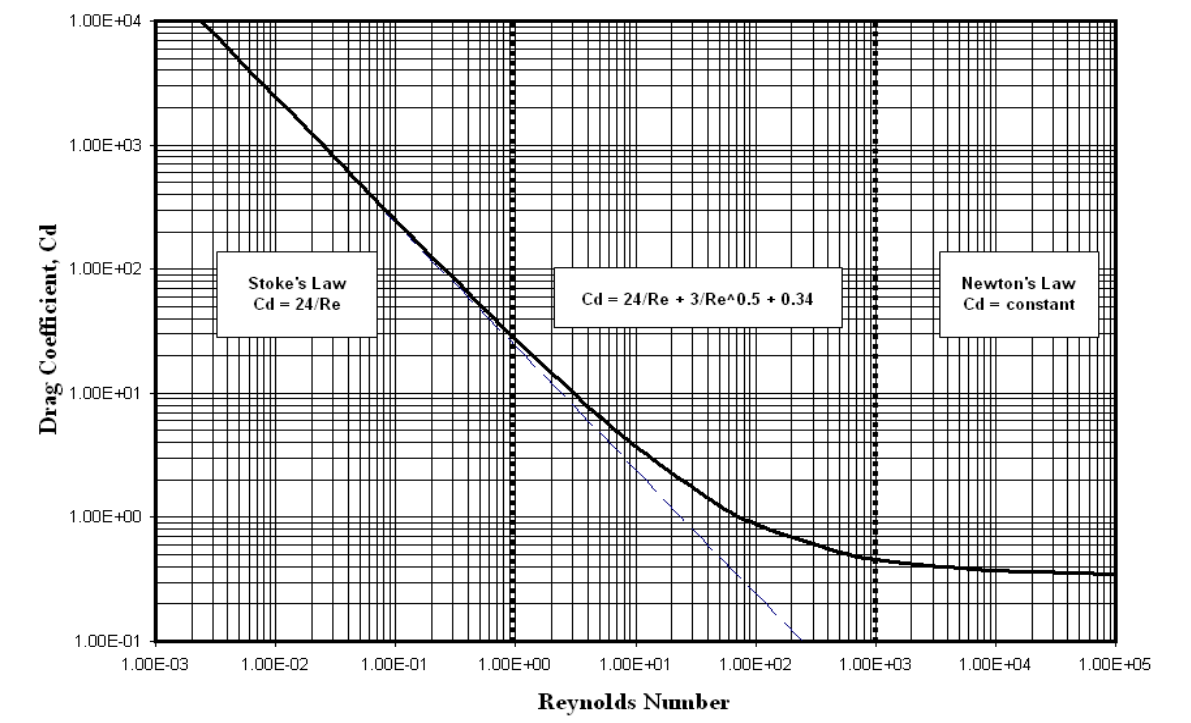
\includegraphics[scale=0.2]{pics/dragRe.png}
			\\{\tiny \justifying Taken from API Specifications for Oil and Gas Separators and PNG 480 Handout. L. Ayala, H. Emami-M. }
		\end{figure}
	\end{frame}
	
	\begin{frame}[t]{Considerations}
		\justifying
		
		\begin{columns}[T]
			
			\column{0.45\textwidth}
			\textbf{Goal}~\\
			\justifying
			
			Test the pseudopotential approach for partially misc. mixtures, under the action of gravity.\\~\\
			
			\textbf{Methodology}~\\
			Test different flow regimes based on Bond (Eotvos) and Morton numbers. Validate against \textbf{terminal velocities and bubble shapes.}
			
			\begin{equation*}
				R_e = \frac{\rho_l u_b d_b}{\mu_l}
			\end{equation*}
			\begin{equation*}
				B_o = \frac{g \Delta \rho d_b^2}{\sigma} \,\,\,\, 	M_o = \frac{g \Delta \rho \mu_l^4}{\sigma^3 
					\rho_l^2}
			\end{equation*}
			
			
			A thermodynamic state fixes $\rho, \Delta \rho, \sigma$. At a given temperature, in a single component case, some values are provided ($\rho, \Delta \rho$) and others can be obtained by simulating the static droplet ($\sigma$). \\
			
			\column{0.45\textwidth}{
				\justifying
				
			}
			
			\textbf{Procedure}	
			\begin{itemize}
				\item Select $B_o$
				\item Calculate the gravity $g = \frac{B_o \sigma}{\Delta \rho d_b^2}$
				\item Select $M_o$
				\item Calculate $\mu_l^4 = \frac{M_o \sigma^3 \rho_l^2}{g \Delta \rho }$
				\item Select the viscosity ratio
				\item Calculate $\mu_g = \mu_l * \frac{\mu_g}{\mu_l}$
			\end{itemize}
			
			The LBM parameters are thus fixed:
			
			\begin{equation*}
				\begin{split}
					\tau = \frac{\nu}{c_s^2}+ \frac{\Delta t}{2}
				\end{split}
			\end{equation*}
			
			\textbf{Try single component and then the multicomponent case.}
		\end{columns}
	\end{frame}
	
	\begin{frame}[t]{Simulation setup (Amaya)}
		\justifying
		\begin{columns}[t]
			\column{0.45\textwidth}
			
			\textbf{Domain}: (!) 200x360 mesh (2D)\\
			\textbf{Fluid}: Water at 485.33 K ($T_r$ = 0.75), and $P_r$ = 0.092. \\$\rho_l^0$  = 7.679 (), $\rho_v^0$  = 0.109. $\rho_L/\rho_g$ = 70. $\tau_l$ = 210.5. $\tau_g$ = 0.8. $\mu_l/\mu_g$ =10.\\~\\
			Initial condition: Spherical droplet with $d_o$ = 40, and $w_o$ = 8.
			
			~\\
			\textbf{Boundary conditions}: No-slip condition on all boundaries.
			
			~\\
			\textbf{Parameters}: Shan-Chen $G$=-1.0. \\
			Beta = 0.9\\
			Time = 10000 ($\approx 10 \sqrt{\frac{d_b}{g}}$)\\
			~\\
			
			
			
			\column{0.45\textwidth}
			
			
			\textbf{Single static simulation}:\\ $\Delta \rho $ = 7.2 (7.7-0.5), $d_s$ = 40.0, \\ $\Delta P$ = 8.5e-3 - 5.87e-3 = 2.623e-3 \\$\sigma = \Delta P \cdot r$ = 0.05254.\\
			
			
			First, the single component case was tested as follows:
			\begin{enumerate}
				\item $B_o$ = 1. $M_o$ = 3e-5. $\mu_R$ = 100. 
				\item $B_o$ = 10. $M_o$ = 2e-2. $\mu_R$ = 10.
				\item $B_o$ = 10. $M_o$ = 2e-2. $\mu_R$ = 100. 
				\item $B_o$ = 0.1. $M_o$ = 1e-2. $\mu_R$ = 100.
				\item $B_o$ = 22. $M_o$ = 8.4e-4. $\mu_R$ = 100. 
			\end{enumerate}
		\end{columns}
	\end{frame}
	
	\begin{frame}{Preliminary Results}
		\begin{figure}
			\centering
			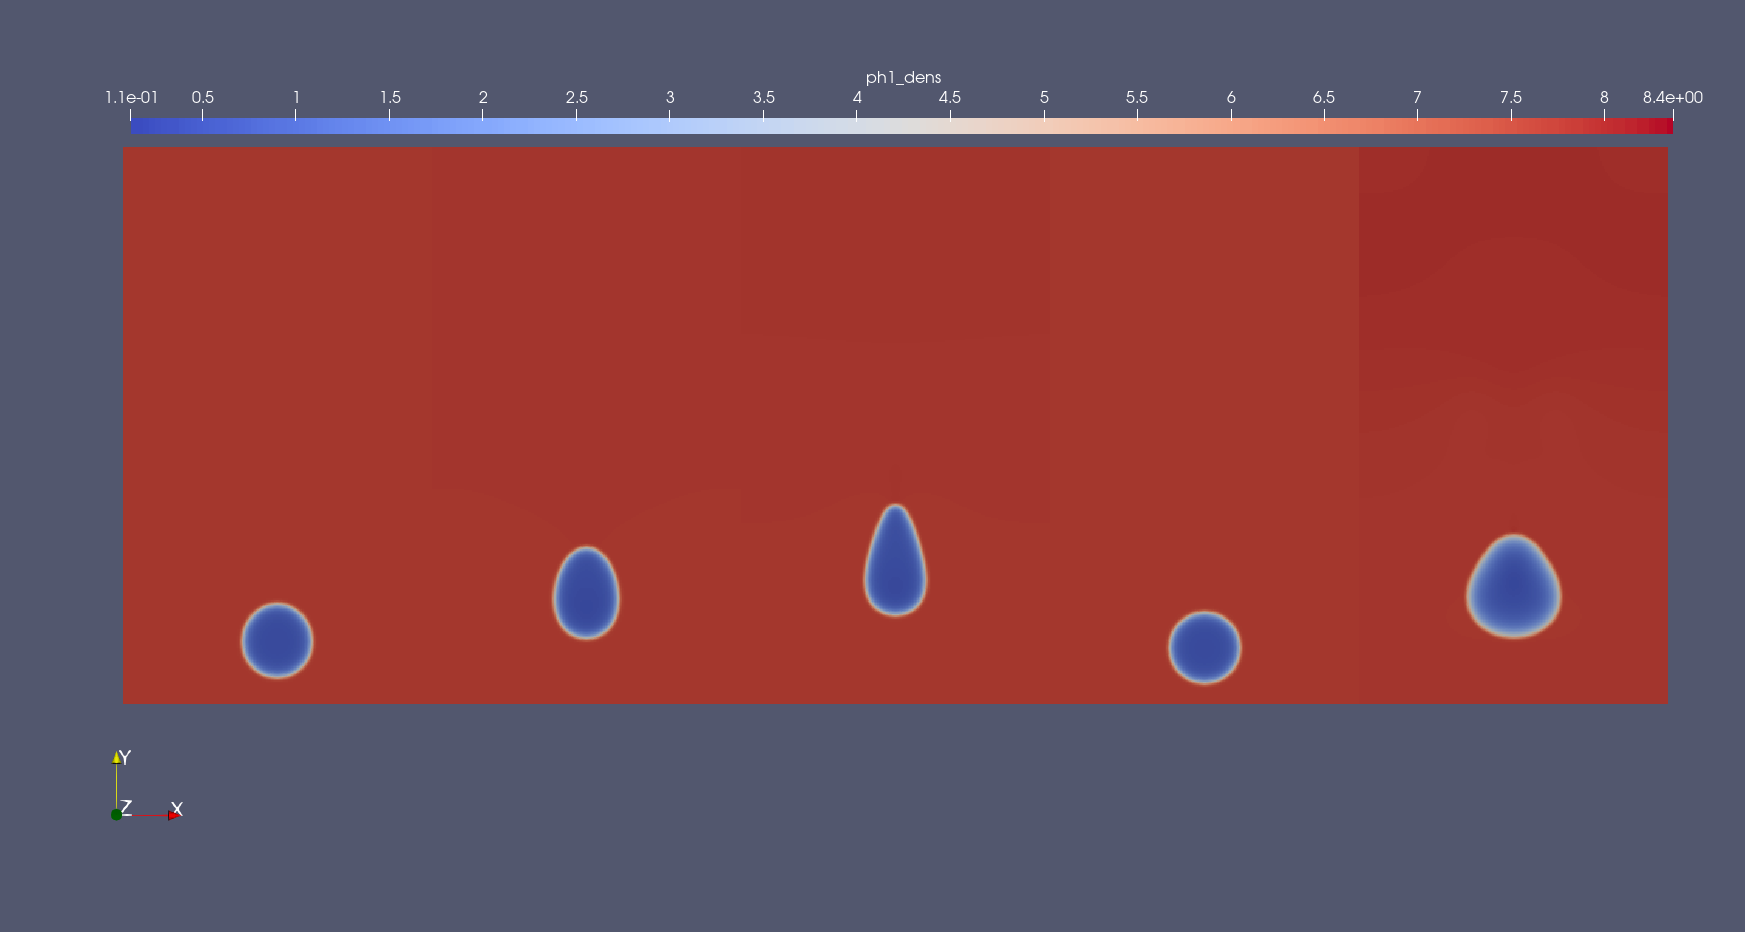
\includegraphics[scale=0.2]{pics/risingCompDen.png}
			\\{\tiny \justifying Bubble shapes}
		\end{figure}
	\end{frame}
	
	\begin{frame}{Preliminary Results}
		\begin{figure}
			\centering
			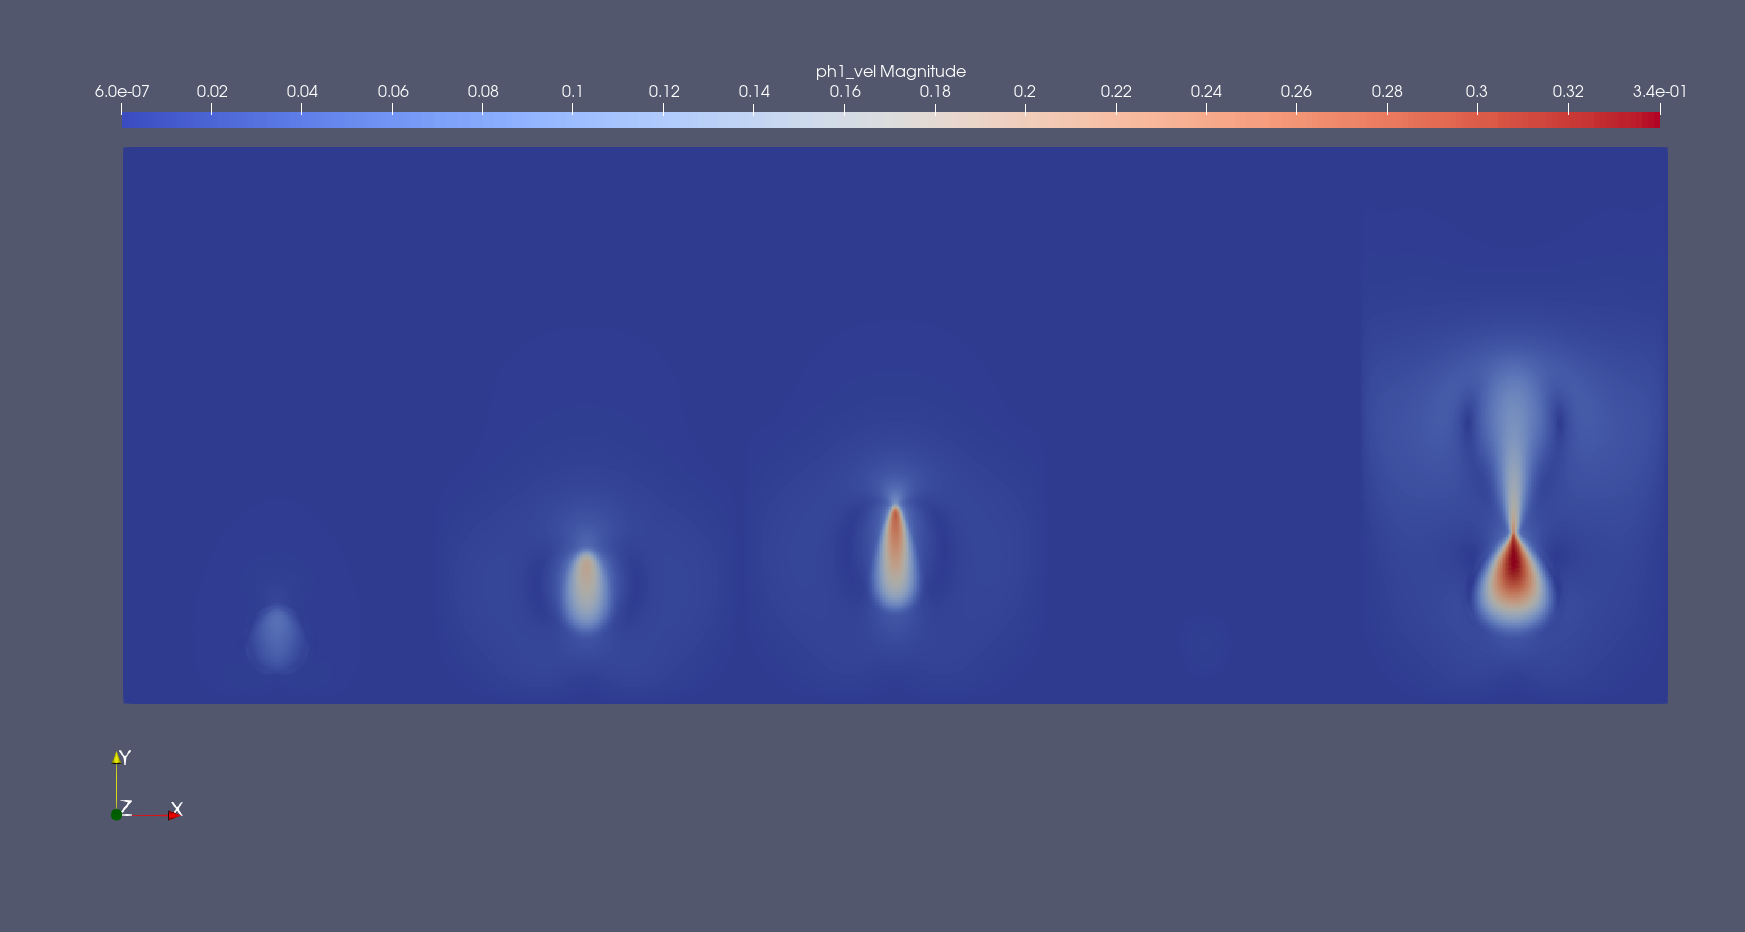
\includegraphics[scale=0.2]{pics/risingCompVel.png}
			\\{\tiny \justifying Velocity field}
		\end{figure}
	\end{frame}
	
	\begin{frame}{Difficulties in single phase}
		\textbf{}\\~\\
		\begin{itemize}
			\item Reach low Morton values (due to restrictions in kinematic viscosity).
			\item Reach high Bond numbers (high gravity)
			\item The cap shapes are not being observed, and the ellipsoidal tends to be more triangular.
			\item Hard to change Bond with fixed $\sigma$. System becomes unstable with other values of $G$.
		\end{itemize}
	\end{frame}
	
	
	\begin{frame}{Increasing the Morton number}
		Trying to make the liquid more viscous (at $B_o$ = 10), seems to not allow the bubble to rise ($M_o$ = 8e6), which later collapses.\\~\\
		\begin{itemize}
			\item $\tau_g$ = 0.52. $\tau_l$ = 47
			\item $\tau_g$ = 2.0. $\tau_l$ = 47 
			\item $\tau_g$ = 0.92. $\tau_l$ = 4.7 
		\end{itemize}
		\begin{figure}
			\centering
			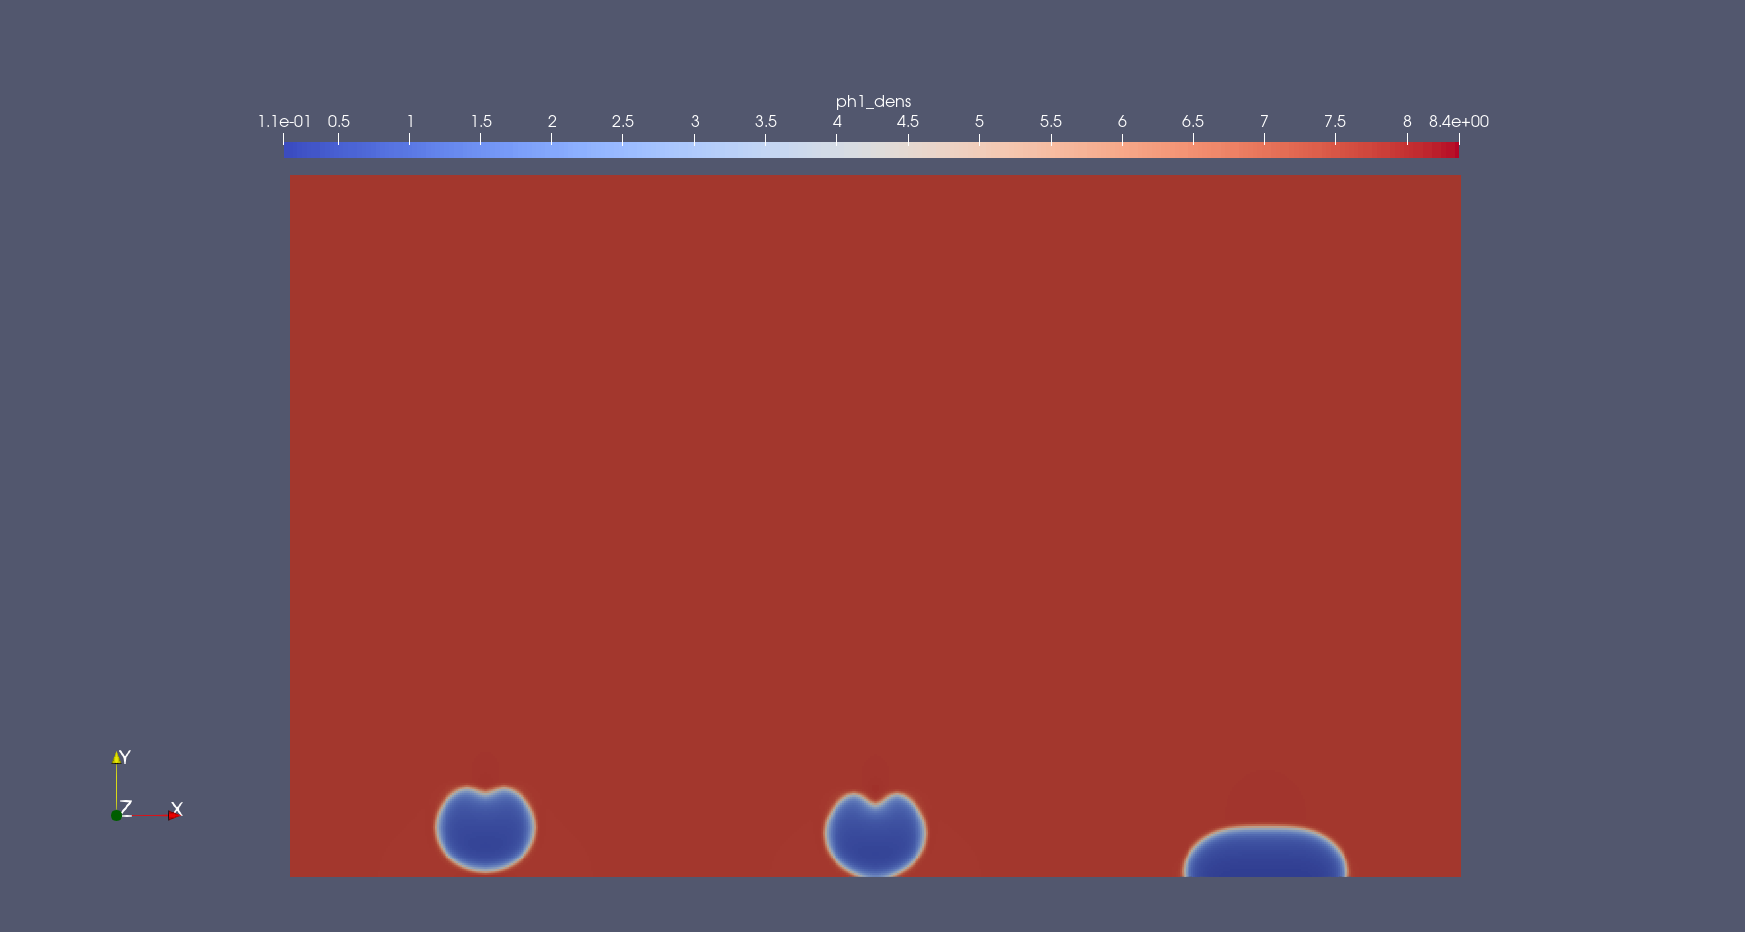
\includegraphics[scale=0.15]{pics/risingCompDen456.png}
			\\{\tiny \justifying Velocity field}
		\end{figure}
	\end{frame}
	
	\begin{frame}{Potential solutions}
		\textbf{}\\~\\
		\begin{itemize}
			\item Fix MRT parameters
			\item Consider an implicit scheme
			\item Compare against the usual Shan-Chen force which may provide better stability 
		\end{itemize}
	\end{frame}
	
	\begin{frame}{Multicomponent case - First approach}
		\textbf{MC case with the beta model}\\~\\
		Using the same mixture that was used for the oscillating droplet, with a viscosity ratio of 10, two cases were run:
		\begin{itemize}
			\item $B_o$ = 10, $M_o$ = 5e-3.
			\item $B_o$ = 10, $M_o$ = 5e-4.
		\end{itemize}
	\end{frame}
	\begin{frame}{Multicomponent case - First approach}
		\begin{figure}
			\centering
			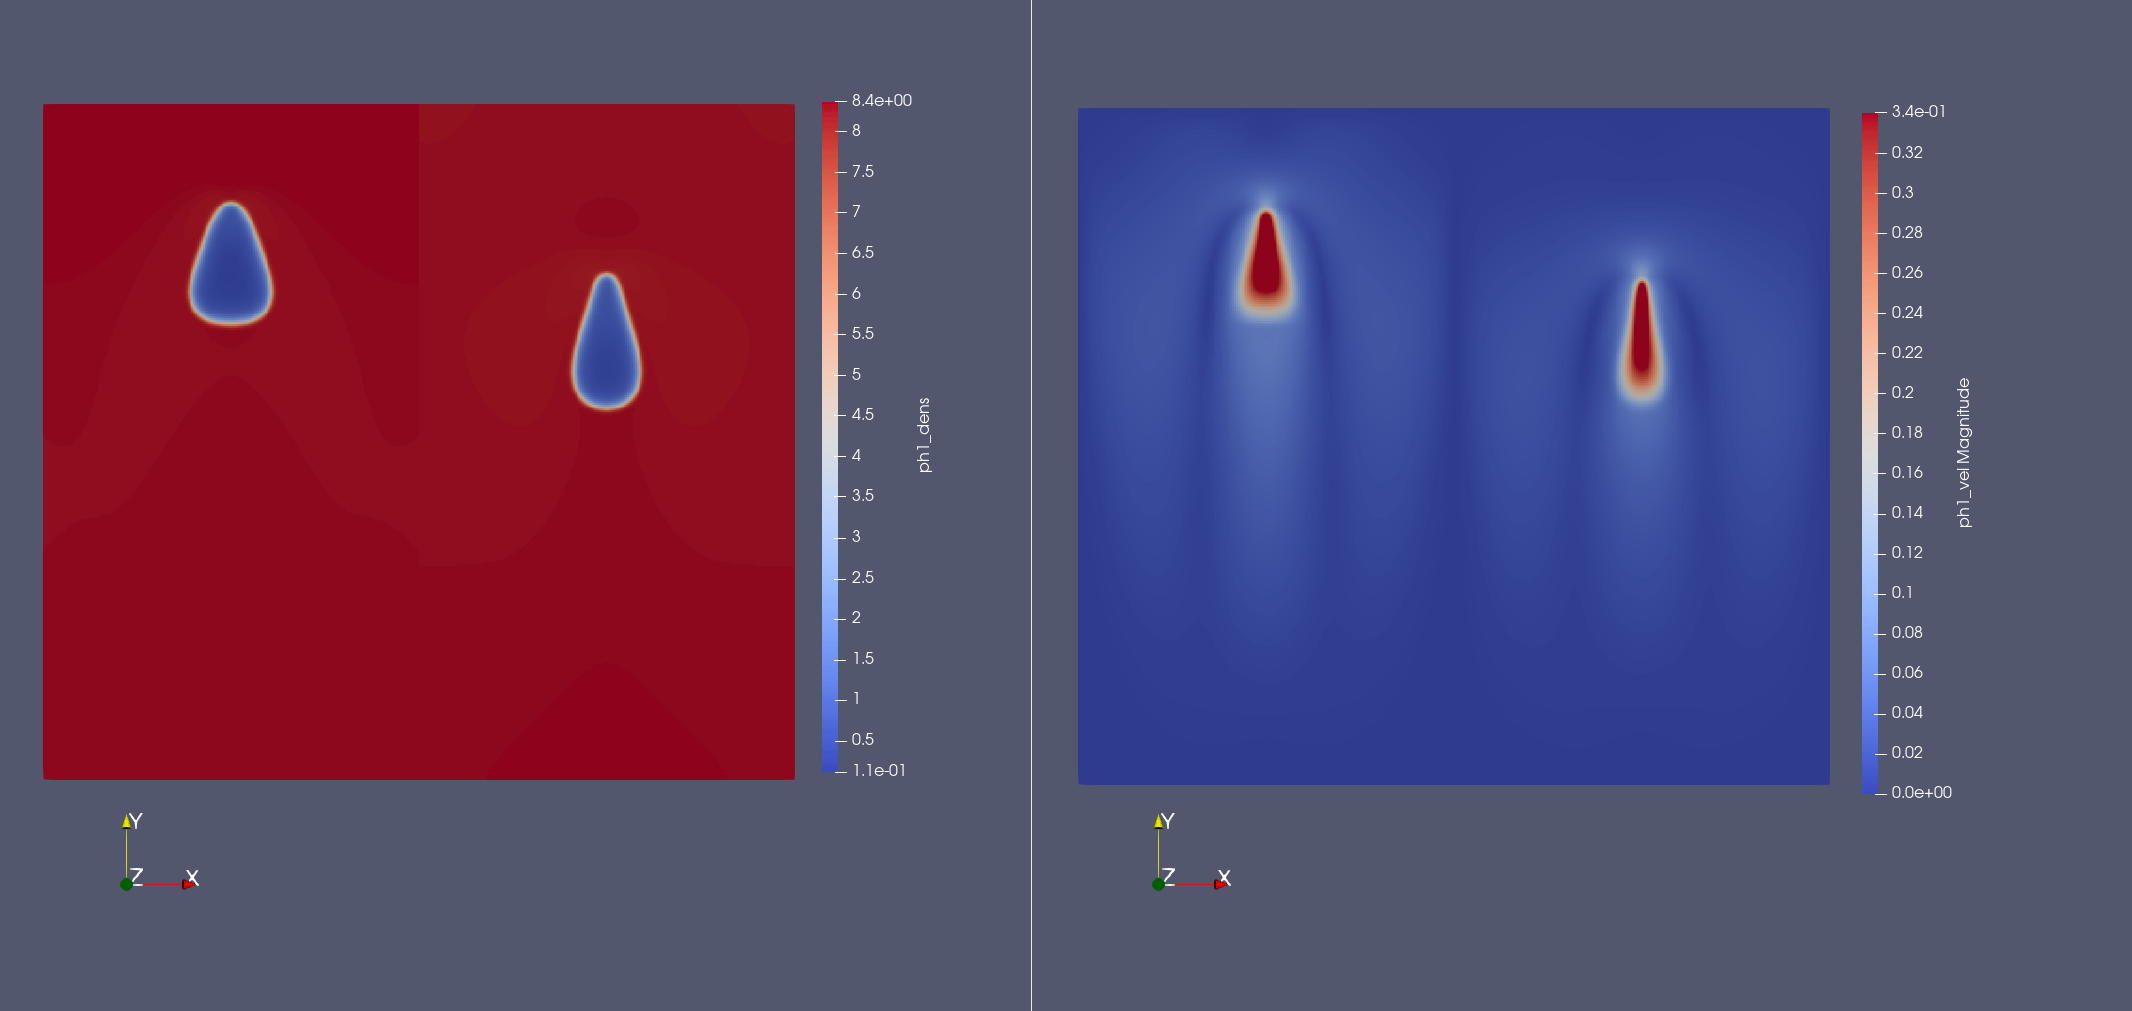
\includegraphics[scale=0.15]{pics/risingMCComp.png}
			\\{\tiny \justifying Density and Velocity field}
		\end{figure}
	\end{frame}
	
	\begin{frame}{Difficulties in single phase}
		\textbf{}\\~\\
		\begin{itemize}
			\item Same as in single component
			\item Reach stable simulations
			\item Seems that walls are affecting more the shape than in the single component
		\end{itemize}
	\end{frame}
	
	\begin{frame}{}
		\centering
		Thank you!
	\end{frame}


	
	
\end{document}